\begin{tiny}(Eee09)\end{tiny}
 \textbf{Les cinq polyèdres réguliers en dimension trois}.\newline
L'objectif de cet exercice n'est pas de construire ces polyèdres mais seulement de faire comprendre pourquoi il n'y en a que cinq.
\begin{figure}[ht]
   \centering
   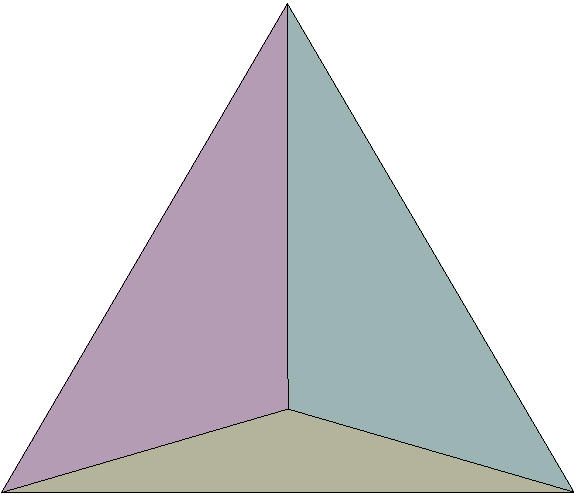
\includegraphics[scale=0.25]{Eee09_1.pdf}
   \caption{tétraèdre}
   \label{fig:1}
\end{figure}

\begin{figure}[ht]
   \centering
   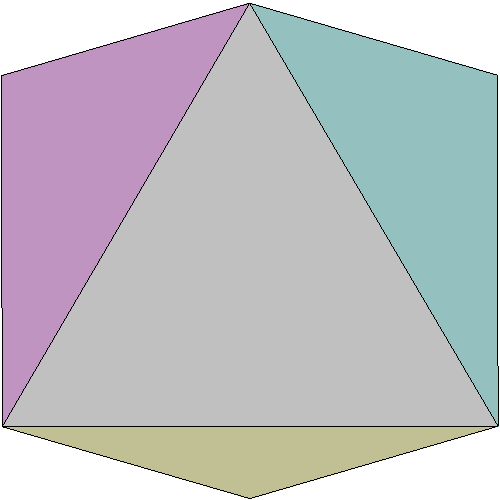
\includegraphics[scale=0.25]{Eee09_2.pdf}
   \caption{octaèdre}
   \label{fig:2}
\end{figure}

\begin{figure}[ht]
   \centering
   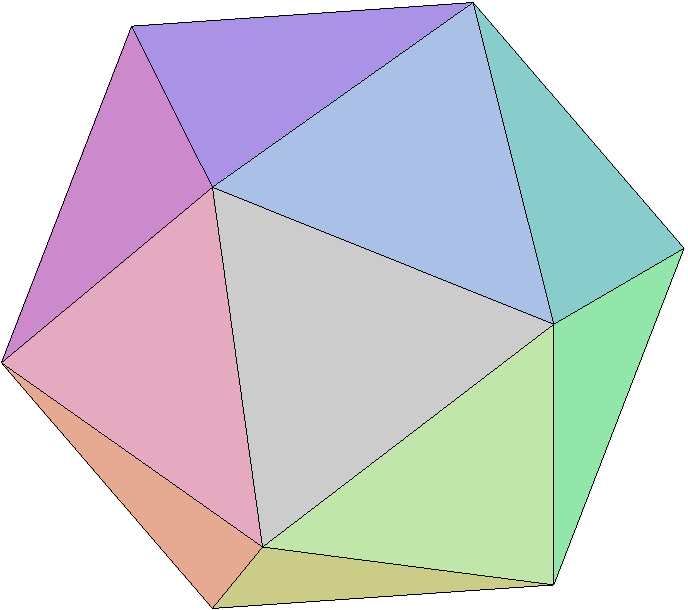
\includegraphics[scale=0.25]{Eee09_3.pdf}
   \caption{icosaèdre}
   \label{fig:3}
\end{figure}

\begin{figure}[ht]
   \centering
   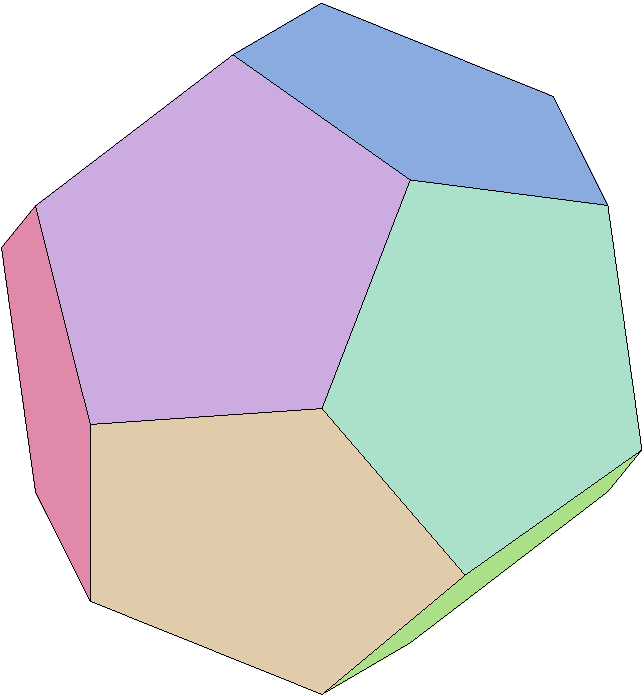
\includegraphics[scale=0.25]{Eee09_4.pdf}
   \caption{dodécaèdre}
   \label{fig:4}
\end{figure}
\begin{figure}
   \centering
   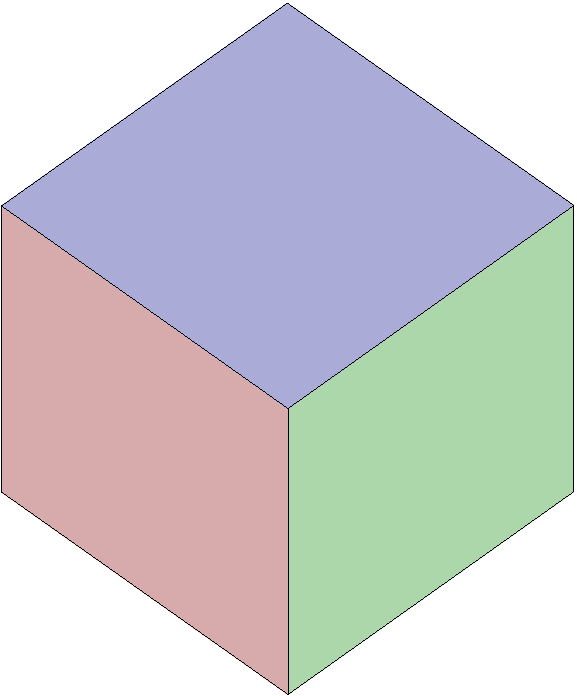
\includegraphics[scale=0.25]{Eee09_5.pdf}
   \caption{cube}
   \label{fig:5}
\end{figure}
Soit $\overrightarrow{u}, \overrightarrow{v}, \overrightarrow{w}$ trois vecteurs unitaires.\newline
On note $\alpha$ l'écart angulaire entre $\overrightarrow{v}$ et $\overrightarrow{w}$, $\beta$ l'écart angulaire entre $\overrightarrow{w}$ et $\overrightarrow{u}$, $\gamma$ l'écart angulaire entre $\overrightarrow{u}$ et $\overrightarrow{v}$.\newline
On suppose $(\overrightarrow{u} / \overrightarrow{w})$ et $(\overrightarrow{v} / \overrightarrow{w})$ strictement positifs.\newline
Soit $p$ la projection orthogonale sur le plan orthogonal à $\overrightarrow{w}$ et $\theta$ l'écart angulaire entre $p(\overrightarrow{u})$ et $p(\overrightarrow{v})$  (faire un dessin).
\begin{enumerate}
\item \begin{enumerate}
  \item   Exprimer $\Vert p(\overrightarrow{u})\Vert$ et $\Vert p(\overrightarrow{v})\Vert$ à l'aide de $\alpha$ et $\beta$.
  \item Trouver une formule reliant $\cos \theta$ et $\cos\gamma$ et faisant intervenir $\alpha$ et $\beta$.
  \item Montrer que $\alpha=\beta$ entraîne $\cos \theta < \cos \gamma$ puis $\theta > \gamma$.
      \end{enumerate}
\item Calculer l'angle entre deux côtés d'un polygone plan régulier à $p$ côtés.
\item On note $p$ le nombre de sommets par face d'un polyèdre régulier et $q$ le nombre de faces autour d'un sommet. Le couple $(p,q)$ est appelé le \emph{symbole de Schlafli} du polyèdre. On se propose de montrer que seuls 5 couples $(p,q)$ sont possibles. En utilisant une projection bien choisie, montrer que
\[q(1-\frac{2}{p}) \pi< 2\pi\]
En déduire
\[(p-2)(q-2)<4\]
Former les 5 couples possibles et les associer aux figures proposées.
\end{enumerate}
